\documentclass[a4paper,12pt]{article}
\usepackage[margin=1in]{geometry} % Set 1-inch margins (adjust as needed)
\usepackage{graphicx}

\title{Practical Work 1: TCP File Transfer}
\author{}
\date{}

\begin{document}

\maketitle

\section*{1. Protocol Design}
The protocol for the file transfer uses the following steps:
\begin{enumerate}
    \item The client connects to the server using a socket.
    \item The client sends a command to the server: \texttt{upload}, \texttt{download}, or \texttt{exit}.
    \item For file upload:
    \begin{itemize}
        \item The client sends the file name and file data in chunks.
        \item The server receives the data and writes it to a file on the server.
    \end{itemize}
    \item For file download:
    \begin{itemize}
        \item The client requests a file.
        \item The server sends the file data in chunks if the file exists.
    \end{itemize}
    \item The session ends when the client sends the \texttt{exit} command.
\end{enumerate}

\noindent \textbf{Figure: Protocol Design Diagram}
\begin{figure}[h!]
    \centering
    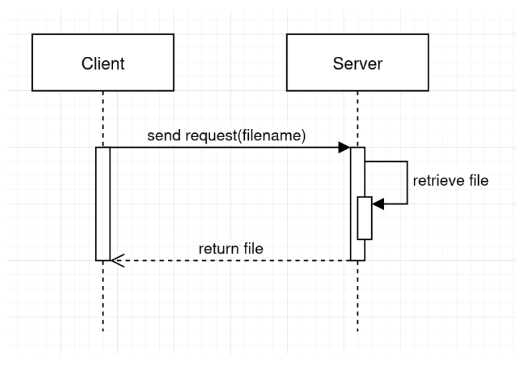
\includegraphics[width=0.8\textwidth]{protocal_figure.png} % Replace with your image path
    \caption{Client-Server Interaction Protocol}
\end{figure}

\section*{2. System Organization}
The system consists of two components:
\begin{enumerate}
    \item \textbf{Server:}
    \begin{itemize}
        \item Initializes a socket.
        \item Waits for a connection from a client.
        \item Handles commands from the client (upload, download, exit).
    \end{itemize}
    \item \textbf{Client:}
    \begin{itemize}
        \item Connects to the server using a socket.
        \item Sends commands and file data to the server.
        \item Receives file data from the server.
    \end{itemize}
\end{enumerate}

\noindent \textbf{Figure: System Organization Diagram}
\begin{figure}[h!]
    \centering
    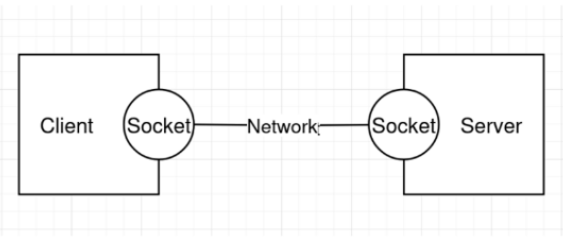
\includegraphics[width=0.8\textwidth]{system.png} % Replace with your image path
    \caption{System Architecture}
\end{figure}

\section*{3. Implementation of File Transfer}
The implementation was divided into the following tasks:
\begin{enumerate}
    \item \textbf{Server Implementation:} The server is responsible for initializing the socket, accepting connections, and handling client commands.
    \item \textbf{Client Implementation:} The client is responsible for connecting to the server, sending commands, and managing file transfers.
    \item \textbf{Protocol Handling:} Defined the commands and their corresponding actions, such as upload, download, and exit.
\end{enumerate}

\section*{4. Team Contributions}
The tasks were distributed as follows among the five team members:
\begin{itemize}
    \item \textbf{Protocol Design:} Do Thi Huong Tra (BA12-174) and Vu Hoang Mai Nhi (22BI13352)
    \item \textbf{Server Code Implementation:} Cao Nhat Nam (22BI13320)
    \item \textbf{Client Code Implementation:} Pham Ngoc Minh Chau (22BI13063)
    \item \textbf{Report Writing and Final Compilation:} Bui Nguyen Ngoc Huyen (22BI13199)
\end{itemize}

\end{document}
